%----------------------------------------------------------------
%
%  File    :  thesis.tex
%
%  Authors :  Keith Andrews, IICM, TU Graz, Austria
%             Manuel Koschuch, FH Campus Wien, Austria
%			  Sebastian Ukleja, FH Campus Wien, Austria
% 
%  Created :  22 Feb 96
% 
%  Changed :  14 Oct 2020
%
%  For suggestions and remarks write to: sebastian.ukleja@fh-campuswien.ac.at 
%----------------------------------------------------------------

% --- Setup for the document ------------------------------------

%Class for a book like style:
\documentclass[11pt,a4paper,oneside]{scrbook}
%For a more paper like style use this class instead:
%\documentclass[11pt,a4paper,oneside]{thesis}

%input encoding for windows in utf-8 needed for Ä,Ö,Ü etc..:
\usepackage[utf8]{inputenc}
%input encoding for linux:
%\usepackage[latin1]{inputenc}
%input encoding for mac:
%\usepackage[applemac]{inputenc}

\usepackage[ngerman]{babel}
\hyphenation{Lifecycle}
\hyphenation{ViewModel}
\hyphenation{LiveData}
\hyphenation{Paging}
\hyphenation{DataStore}
\hyphenation{Room }
\hyphenation{WorkManager}
\hyphenation{Navigation}

%for english use this instead:
%\usepackage[english]{babel}

\usepackage{csquotes}
\MakeOuterQuote{"}

\usepackage{float}

\usepackage{minted}

%needed for font encoding
\usepackage[T1]{fontenc}

% want Arial? uncomment next two lines...
%\usepackage{uarial}
%\renewcommand{\familydefault}{\sfdefault}

%some formatting packages
\usepackage[bf,sf]{subfigure}
\renewcommand{\subfigtopskip}{0mm}
\renewcommand{\subfigcapmargin}{0mm}

%For better font resolution in pdf files
\usepackage{lmodern}

\usepackage{url}

%\usepackage{latexsym}

\usepackage{geometry} % define pagesize in more detail

% --- Settings for header and footer ---------------------------------
\usepackage{scrlayer-scrpage}
\clearscrheadfoot
\pagestyle{scrheadings}
\automark{chapter}

%Left header shows chapter and chapter name, will not display on first chapter page use \ihead*{\leftmark} to show on every page
\ihead{\leftmark} 	
%\ohead*{\rightmark}	%optional right header
\ifoot*{Markus Mayer}	%left footer shows student name
\ofoot*{\thepage}		%right footer shows pagination
%---------------------------------------------------------------------

\usepackage{colortbl} % define colored backgrounds for tables

\usepackage{courier} %for listings
\usepackage{listings} % nicer code formatting
\lstset{basicstyle=\ttfamily,breaklines=true,breakatwhitespace}
\let\oldlstinline\lstinline
\renewcommand{\lstinline}[1]{\sloppy\oldlstinline{#1}}

\usepackage[dvipsnames]{xcolor}

\definecolor{groovyblue}{HTML}{0000A0}
\definecolor{groovygreen}{HTML}{008000}
\definecolor{darkgray}{rgb}{.4,.4,.4}
 
\lstdefinelanguage{Groovy}[]{Java}{
  keywordstyle=\color{groovyblue}\bfseries,
  stringstyle=\color{groovygreen}\ttfamily,
  keywords=[3]{each, findAll, groupBy, collect, inject, eachWithIndex},
  morekeywords={def, as, in, use},
  moredelim=[is][\textcolor{darkgray}]{\%\%}{\%\%},
  moredelim=[il][\textcolor{darkgray}]{§§}
}

\lstdefinelanguage{Kotlin}{
  comment=[l]{//},
  commentstyle={\color{gray}\ttfamily},
  emph={filter, first, firstOrNull, forEach, lazy, map, mapNotNull, println},
  emphstyle={\color{OrangeRed}},
  identifierstyle=\color{black},
  keywords={!in, !is, abstract, actual, annotation, as, as?, break, by, catch, class, companion, const, constructor, continue, crossinline, data, delegate, do, dynamic, else, enum, expect, external, false, field, file, final, finally, for, fun, get, if, import, in, infix, init, inline, inner, interface, internal, is, lateinit, noinline, null, object, open, operator, out, override, package, param, private, property, protected, public, receiveris, reified, return, return@, sealed, set, setparam, super, suspend, tailrec, this, throw, true, try, typealias, typeof, val, var, vararg, when, where, while},
  keywordstyle={\color{NavyBlue}\bfseries},
  morecomment=[s]{/*}{*/},
  morestring=[b]",
  morestring=[s]{"""*}{*"""},
  ndkeywords={@Deprecated, @JvmField, @JvmName, @JvmOverloads, @JvmStatic, @JvmSynthetic, Array, Byte, Double, Float, Int, Integer, Iterable, Long, Runnable, Short, String, Any, Unit, Nothing},
  ndkeywordstyle={\color{BurntOrange}\bfseries},
  sensitive=true,
  stringstyle={\color{ForestGreen}\ttfamily},
}

\usepackage{graphicx}
  \pdfcompresslevel=9
  \pdfpageheight=297mm
  \pdfpagewidth=210mm
  \usepackage[         % hyperref should be last package loaded
    pdftex, 		   % needed for pdf compiling, DO NOT compile with LaTeX
    bookmarks,
    bookmarksnumbered,
    linktocpage,
    pagebackref,
    pdfview={Fit},
    pdfstartview={Fit},
    pdfpagemode=UseOutlines,                 % open bookmarks in Acrobat
  ]{hyperref}
\DeclareGraphicsExtensions{.pdf,.jpg,.png}
\usepackage{bookmark}

\usepackage[title]{appendix}

\usepackage{caption}

\usepackage{varwidth}
\DeclareCaptionFormat{myformat}{%
  % #1: label (e.g. "Table 1")
  % #2: separator (e.g. ": ")
  % #3: caption text
  \begin{varwidth}{\linewidth}%
    \centering
    #1#2#3%
  \end{varwidth}%
}
\captionsetup{format=myformat}

%paper format
\geometry{a4paper,left=30mm,right=25mm, top=30mm, bottom=30mm}

\setlength{\parskip}{3pt plus 1pt minus 0pt}       % vert. space before a paragraph

\setcounter{tocdepth}{1}        % lowest section level entered in ToC
\setcounter{secnumdepth}{2}     % lowest section level still numbered

%Start of your document beginning with title page
\begin{document}

% --- Main Title Page ------------------------------------------------
\begin{titlepage}
\frontmatter
\begin{picture}(50,50)
\put(-70,40){\hbox{
\includegraphics{images/logo.png}}}
\end{picture}

\vspace*{-5.8cm}

\begin{center}

\vspace{6.2cm}

\hspace*{-1.0cm} {\LARGE \textbf{Android Jetpack Architecture Komponenten \\}}
\vspace{0.2cm}
\hspace*{-1.0cm} Ein Überblick \\

\vspace{2.0cm}

\hspace*{-1.0cm} { \textbf{Bachelorarbeit\\}}

\vspace{0.65cm}

\hspace*{-1.0cm} Eingereicht in teilweiser Erfüllung der Anforderungen zur Erlangung des akademischen Grades: \\

\vspace{0.65cm}

\hspace*{-1.0cm} \textbf{Bachelor of Science in Engineering\\}

\vspace{0.65cm}

\hspace*{-1.0cm} an der FH Campus Wien \\
\vspace{0.2cm}
\hspace*{-1.0cm} Studienfach: Computer Science and Digital Communications \\

\vspace{1.6cm}

\hspace*{-1.0cm} \textbf{Autor:} \\
\vspace{0.2cm}
\hspace*{-1.0cm} Markus Mayer \\

\vspace{0.7cm}

\hspace*{-1.0cm} \textbf{Matrikelnummer:}\\
\vspace{0.2cm}
\hspace*{-1.0cm} 52006537 \\

\vspace{0.7cm}

\hspace*{-1.0cm} \textbf{Betreuer:} \\
\vspace{0.2cm}
\hspace*{-1.0cm} René Goldschmid, MSc \\

\vspace{0.7cm}

% Reviewer if needed:
%\hspace*{-1.0cm} \textbf{Reviewer: (optional)} \\
%\vspace{0.2cm}
%\hspace*{-1.0cm} Titel Vorname Nachname \\


\vspace{1.0cm}

\hspace*{-1.0cm} \textbf{Datum:} \\
\vspace{0.2cm}
\hspace*{-1.0cm} 15.01.2023 \\

\end{center}
\end{titlepage}

\newpage

\setcounter{page}{1}

\vspace*{16cm}

% --- Declaration of authorship --------------------------------------------
\hspace*{-0.7cm} \underline{Erklärung der Urheberschaft:}\\\\
Ich erkläre hiermit diese Bachelorarbeit eigenständig verfasst zu haben. Ich habe keine anderen Quellen, als die in der Arbeit gelisteten verwendet, noch habe ich jegliche unerlaubte Hilfe in Anspruch genommen\\\\
Ich versichere diese Bachelorarbeit in keinerlei Form jemandem Anderen oder einer anderen Institution zur Verfügung gestellt zu haben, weder in Österreich noch im Ausland.\\\\
Weiters versichere ich, dass jegliche Kopie (gedruckt oder digital) identisch ist.
\\\\\\
Datum: \hspace{6cm} Unterschrift:\\

% --- English Abstract ----------------------------------------------------
\cleardoublepage
\chapter*{Abstract}

Android application development has changed and evolved rapidly over the last few years as the hardware offers more and more possibilities. The smartphone has become a multifunctional tool and therefore not only the number of available applications has increased, but also the complexity of certain applications to be able to use various functions. This leads to higher demands on the developers of Android applications. To cope with complex applications, developers need a tool to work more efficiently. With Android Jetpack a collection of components was published, which should simplify application development and reduce the quantity of written code. 

Therefore, this paper takes a closer look at the Architecture components of Android Jetpack, which consist of Lifecycle, ViewModel, LiveData, Paging, DataStore, Room, WorkManager and Navigation, and explains their possibilities and advantages. After taking a closer look at the individual Android Jetpack Architecture components, it can be confirmed that it is possible to develop applications easier and more efficiently. In this bachelor thesis, a literature search was performed. As sources, books, papers, and online sources, such as the official documentation and the Android Developers Blog, were used. 


% --- German Abstract ----------------------------------------------------

\cleardoublepage
\chapter*{Kurzfassung}

Die Entwicklung von Android Applikationen hat sich in den letzten Jahren rasch verändert und weiterentwickelt, da die Hardware immer mehr Möglichkeiten bietet. Das Smartphone hat sich zu einem multifunktionalen Werkzeug entwickelt und daher ist nicht nur die Anzahl der verfügbaren Applikationen gestiegen, sondern auch die Komplexität bestimmter Applikationen, um die verschiedensten Funktionen nutzen zu können. Dies führt zu höheren Anforderungen an die Entwickler*innen von Android Applikationen. Um komplexen Applikationen gewachsen zu sein, benötigen die Entwickler*innen ein Werkzeug, um effizienter arbeiten zu können. Mit Android Jetpack wurde eine Sammlung von Komponenten veröffentlicht, welche die Applikationsentwicklung vereinfachen und die Menge an geschriebenen Code verringern soll. 

Diese Arbeit betrachtet daher die Architecture Komponenten von Android Jetpack, die sich aus den Komponenten Lifecycle, ViewModel, LiveData, Paging, DataStore, Room, WorkManager und Navigation zusammensetzen, näher und erläutert deren Möglichkeiten und Vorteile. Nach genauer Betrachtung der einzelnen Android Jetpack Architecture Komponenten kann bestätigt werden, dass einfacher und effizienter gearbeitet werden kann. Bei dieser Bachelorarbeit wurde eine Literaturrecherche durchgeführt, als Quellen wurden Bücher, Papers und Onlinequellen, wie die offizielle Dokumentation und der Android Developers Blog, verwendet.



% --- Abbrevations ----------------------------------------------------
\newpage\noindent
\chapter*{Abkürzungen}
\vspace{0.65cm}

\begin{table*}[htbp]
		\begin{tabular}{ll}
			OHA      & Open Handset Alliance \\
			OAA      & Open Automotive Alliance \\
            LiPS     & Linux Phone Standards Forum  \\
            OMA      & Open Mobile Alliance \\
            IDE      & Integrated Development Enviroment \\
            DSL      & Domain Specific Language \\
            API      & Application Programming Interface \\
            DAO      & Data Access Object \\
		\end{tabular}
\end{table*}

% --- Key terms ----------------------------------------------------
\newpage
\chapter*{Schlüsselbegriffe}
\vspace{0.65cm}

\begin{itemize}
	\setlength{\itemsep}{0pt}
	\item[] Android-Softwareentwicklung
	\item[] Android Jetpack
	\item[] Architecture Komponenten
	\item[] Lifecycle
	\item[] ViewModel
	\item[] LiveData
	\item[] Paging
	\item[] DataStore
	\item[] Room 
	\item[] WorkManager
	\item[] Navigation
\end{itemize}

% --- Table of contents autogenerated ------------------------------------
\newpage
\tableofcontents

% --- Begin of Thesis ----------------------------------------------------
\mainmatter

\chapter{Einführung}

Die Softwareentwicklung für Android Applikationen hat sich in den letzten Jahren rasant verändert und weiterentwickelt. Der Grund dafür liegt in der ständigen Weiterentwicklung der Hardware, die immer mehr Möglichkeiten bietet. Das Smartphone ist heute aus unserem Alltag nicht mehr wegzudenken und zu einem multifunktionalen Werkzeug geworden, daher ist nicht nur die Anzahl der verfügbaren Applikationen gestiegen, sondern auch die Komplexität bestimmter Applikationen, um die verschiedensten Funktionen zu nutzen. Mit den heutigen Applikationen ist es möglich zu navigieren, zu bezahlen, zu kommunizieren beziehungsweise Gesundheits- und Bewegungsdaten zu speichern und vieles mehr. Das bedeutet jedoch auch für die*den Entwickler*in steigende Anforderungen bei der Entwicklung der Applikationen. Daher bietet Android mit Android Jetpack, Bibliotheken und vereinfachte Ansätze, die eine Erleichterung bei der Erstellung von Android Applikationen bieten. Eine Zusammenfassung der Komponenten ist jedoch zum Zeitpunkt der Arbeit nicht verfügbar. Daher werden in weiterer Folge die Möglichkeiten und Vorteile, die Android Jetpack mit den einzelnen Architecture Komponenten bietet, näher erläutert. 

Die vorliegende Arbeit ist folgendermaßen aufgebaut: Kapitel \ref{chap:Android} gibt einen Überblick über die Entwicklung von Android, die Ziele, die mit der Open-Source-Software angestrebt werden, und den Programmiersprachen, die in Android unterstützt werden, inklusive den Vorteilen der Programmiersprache Kotlin. Die letzten beiden Abschnitte informieren über Android Studio und die Funktionsweise des Gradle Automatisierungstools. Kapitel \ref{chap:androidJetpack-Übersicht} erörtert die Entwicklung von Android Jetpack, wie es der*dem Entwickler*in die Arbeit erleichtert und wie es aufgebaut ist. In Kapitel \ref{chap:androidJetpack-Komponenten} wird das Hinzufügen und die Versionierung von Jetpack-Komponenten erklärt und auf die Architecture Komponenten näher eingegangen. Kapitel \ref{chap:Schluss} fasst die einzelnen Komponenten mit ihren Möglichkeiten zusammen, bringt sie in Verbindung und gibt einen Ausblick auf mögliche weiterführende Arbeiten. 


\chapter{Android}
\label{chap:Android}

Um einen Überblick über Android zu bekommen, beziehungsweise wo der Fokus eines der am weitest verbreitetsten Betriebssysteme für mobile Geräte liegt, muss etwas in die Vergangenheit geblickt werden. Android ist ein Open-Source-Betriebssystem, welches auf einem Linux-Kernel basiert. Es wurde von der Firma Android Inc. entwickelt, die im Jahr 2005 von Google übernommen wurde \cite{hrmoandroid}.


\section{Rückblick}

Im Jahr 2006 hatten Unternehmen, die ein Smartphone auf den Markt bringen wollten, die Möglichkeit, teure Lizenzgebühr für ein Betriebssystem zu bezahlen oder ein eigenes Betriebssystem zu entwickeln. Google gründete 2007 die Open Handset Alliance (OHA) und führte Android als Open Source-Plattform ein. Im Jahr 2008 wurde Android auf die Version mit dem Namen Cupcake aktualisiert. Bei dieser Version können Unternehmen wie HTC und Samsung, aber auch Mobilfunkanbieter das Betriebssystem ihrer Smartphones anpassen. Laut Google kommt 2010 Android auf 34 Mobilgerätetypen in 49 Ländern zum Einsatz und bietet damit den Nutzenden eine größere Auswahl als je zuvor. 2011 veröffentlichte Google mit Android 3.0 Honeycomb ein für Tablets optimiertes Betriebssystem, das als Basis für das Betriebssystem Fire OS des Kindle Fire-Tablets von Amazon dient. Der sogenannte Android Market wurde 2012 in Google Play umbenannt und Entwickler*innen können weiterhin ihre Apps in wenigen Stunden veröffentlichen. Zusätzlich zur Unterstützung von Mobilgeräten wurde 2014 die Open Automotive Alliance (OAA) gegründet, deren Ziel es ist, Android auch für Autos zu nutzen. Zum Zeitpunkt der Arbeit sind 45 führende Automarken Mitglied der OAA. Durch die Innovationskraft einiger Unternehmen sind 2015 inzwischen Android-Geräte für weniger als 50 US-Dollar verfügbar. Mit Stand 2016 gibt es fast 24.000 Android-Geräte von über 1.300 Marken. Außerdem gibt es zum Zeitpunkt der Arbeit dutzende weltweit operierende Stores für Android-Apps. \cite{android.com}


\section{Ziele}

Androids Ziele sind zwar ähnlich zu denen des Linux Phone Standards Forum (LiPS) oder der Open Mobile Alliance (OMA), da aber der Ansatz des kompletten Software-Stacks von Android weit über den Fokus dieser standarddefinierenden Organisationen hinausgeht, ist Android kein Teil dieser Organisationen. Verglichen mit dem iPhone, das eine vollständig herstellungsspezifische Hardware- und Softwareplattform ist, die von einem einzigen Unternehmen herausgegeben wird, ist Android ein Open Source-Software-Stack, der von der OHA entwickelt und unterstützt wird und auf jedem kompatiblen Gerät funktionieren soll. \cite{meier_hello_android}


\section{Unterstützte Programmiersprachen}

Bis 2019 war Java die offizielle Standardprogrammiersprache für die Entwicklung von Android-Apps. Als 2017 Kotlin als unterstützte Sprache für die Android-Entwicklung angekündigt wurde, gab es zu Beginn große Aufregung unter den Entwicklern*innen. Die Anzahl der Entwickler*innen, die Kotlin verwenden, ist jedoch in kürzester Zeit so gestiegen, dass im Jahr 2019 Kotlin, Java als offizielle Standardprogrammiersprache ablöste. \cite{ android_kotlin}

Mit Javas Ablöse als Standardprogrammiersprache wurde seitens Android jedoch weiterhin der offizielle Support für Java und C++ zugesichert \cite{ android_languages}. Das Feedback, das direkt von den Entwicklern*innen kommt, hebt folgende Vorteile bei der Verwendung von Kotlin hervor, wie unter "Android’s Kotlin-first approach" beschrieben wird \cite{developer.android.com/kotlin/first}.

\begin{itemize} 
  \item \textbf{Ausdrucksstark und prägnant} \\ 
        Es kann mit weniger Code mehr erreicht werden. Codesegmente, die ohne Änderung immer wieder verwendet werden, fachsprachlich auch Boilerplate-Code genannt, können merkbar reduziert werden. Somit kann Kotlin die Produktivität der Entwickler*innen erhöhen. 
  \item \textbf{Sicherer Code} \\ 
        Kotlin enthält viele Sprachfunktionen, die dabei helfen, häufige Programmierfehler wie zum Beispiel Null Pointer Exceptions zu vermeiden. Android-Apps mit Kotlin Code haben eine zwanzigprozentige geringere Absturzwahrscheinlichkeit. 
  \item \textbf{Interoperabel} \\ 
        Kotlin ist zu 100 Prozent interoperabel mit der Programmiersprache Java, das heißt, dass Java Code in Kotlin verwendet werden kann und Kotlin Code auch problemlos von Java aus verwendet werden kann. Damit können die Entwickler*innen so viel oder so wenig Kotlin Code in ihren Projekten verwenden, wie sie möchten. 
  \item \textbf{Strukturierte Gleichzeitigkeit} \\ 
        Mit Kotlin Coroutines ist das Arbeiten mit asynchronem Code genauso einfach wie mit blockierendem Code. Diese Coroutines vereinfachen die Verwaltung von diversen Hintergrundaufgaben.
\end{itemize}


\section{Android Studio}

Android Studio ist seit 2013 die offizielle Integrated Development Environment (IDE) von Google für die Android-Softwareentwicklung. Um Android Studio zu entwickeln, ging Google eine Kooperation mit der tschechischen Firma JetBrains ein, die zu diesem Zeitpunkt mit IntelliJ IDEA eine der fortschrittlichsten Java IDEs am Markt hatten und auch heute noch haben. Android Studio basiert auf dieser leistungsstarken Entwicklungsumgebung, die von Google mit speziellen Funktionen für die Android-Entwicklung erweitert und angepasst wurde. Eine dieser Funktionen ist ein Build-System, das auf Gradle basiert und mit dem Android Gradle Plugin um einige Features erweitert wurde. Die aktuelle Version zum Zeitpunkt der Arbeit ist Android Studio Dolphin mit dem Versionscode 2021.3.1. Android Studio ist ein Open-Source-Projekt und steht auch frei zum Download zur Verfügung. \cite{android_studio}

\newpage
\section{Gradle}

Gradle ist ein Build-Management-Automatisierungstool, das den automatischen Download und die Konfiguration von Abhängigkeiten und anderen Bibliotheken übernimmt \cite{Hassan2018}. Gradle stellt im Allgemeinen Standardwerte für Einstellungen und Eigenschaften bereit, daher ist der Einstieg für Entwickler*innen einfacher als bei Systemen wie Ant oder Maven, die davor die Standard Build-Systeme bei Android-Projekten waren. Wenn ein neues Projekt mit Android Studio angelegt wird, werden standardmäßig drei Gradle Files generiert. \cite{Pelgrims2015_1} Die Dateien \lstinline{settings.gradle} und \lstinline{build.gradle} befinden sich im Stammverzeichnis und eine weitere \lstinline{build.gradle} Datei wird im App Ordner angelegt. Die \lstinline{build.gradle} Datei im Stammverzeichnis wirkt sich auf jedes Modul des Projekts aus und die \lstinline{build.gradle} Datei im \lstinline{App} Ordner wirkt sich nur auf das \lstinline{App} Modul aus. In der \lstinline{settings.gradle} Datei werden die Repository-Einstellungen auf Projektebene definiert und Gradle mitgeteilt, welche Module bei Erstellung der Anwendung inkludiert werden sollen. Diese Gradle Dateien werden mit einer Domain Specific Language (DSL) geschrieben, wobei entweder Groovy oder Kotlin verwendet wird. \cite{Pelgrims2015_2}


\chapter{Android Jetpack-Übersicht}
\label{chap:androidJetpack-Übersicht}

Android Jetpack wurde von der Support Library inspiriert. Dabei handelt es sich um eine Reihe von Komponenten, die es erleichtern, neue Android Funktionen zu nutzen und dabei trotzdem eine Abwärtskompatibilität aufrechtzuerhalten. Nahezu jede App im Play Store verwendete diese Support Library. Aufgrund dieser Beliebtheit wurden 2017 die Architecture Komponenten eingeführt. Sie erleichtern den Umgang mit Daten bei Änderungen und Komplikationen im Lebenszyklus einer App. Android Jetpack bringt die existierende Support Library und die Architecture Komponenten zusammen und gliedert sie in vier Kategorien, wie in Abbildung \ref{fig:AndroidJetpackUebersicht} zu sehen ist. \cite{android_jetpack_ueberblick}

\begin{figure}[H]
	\centering
		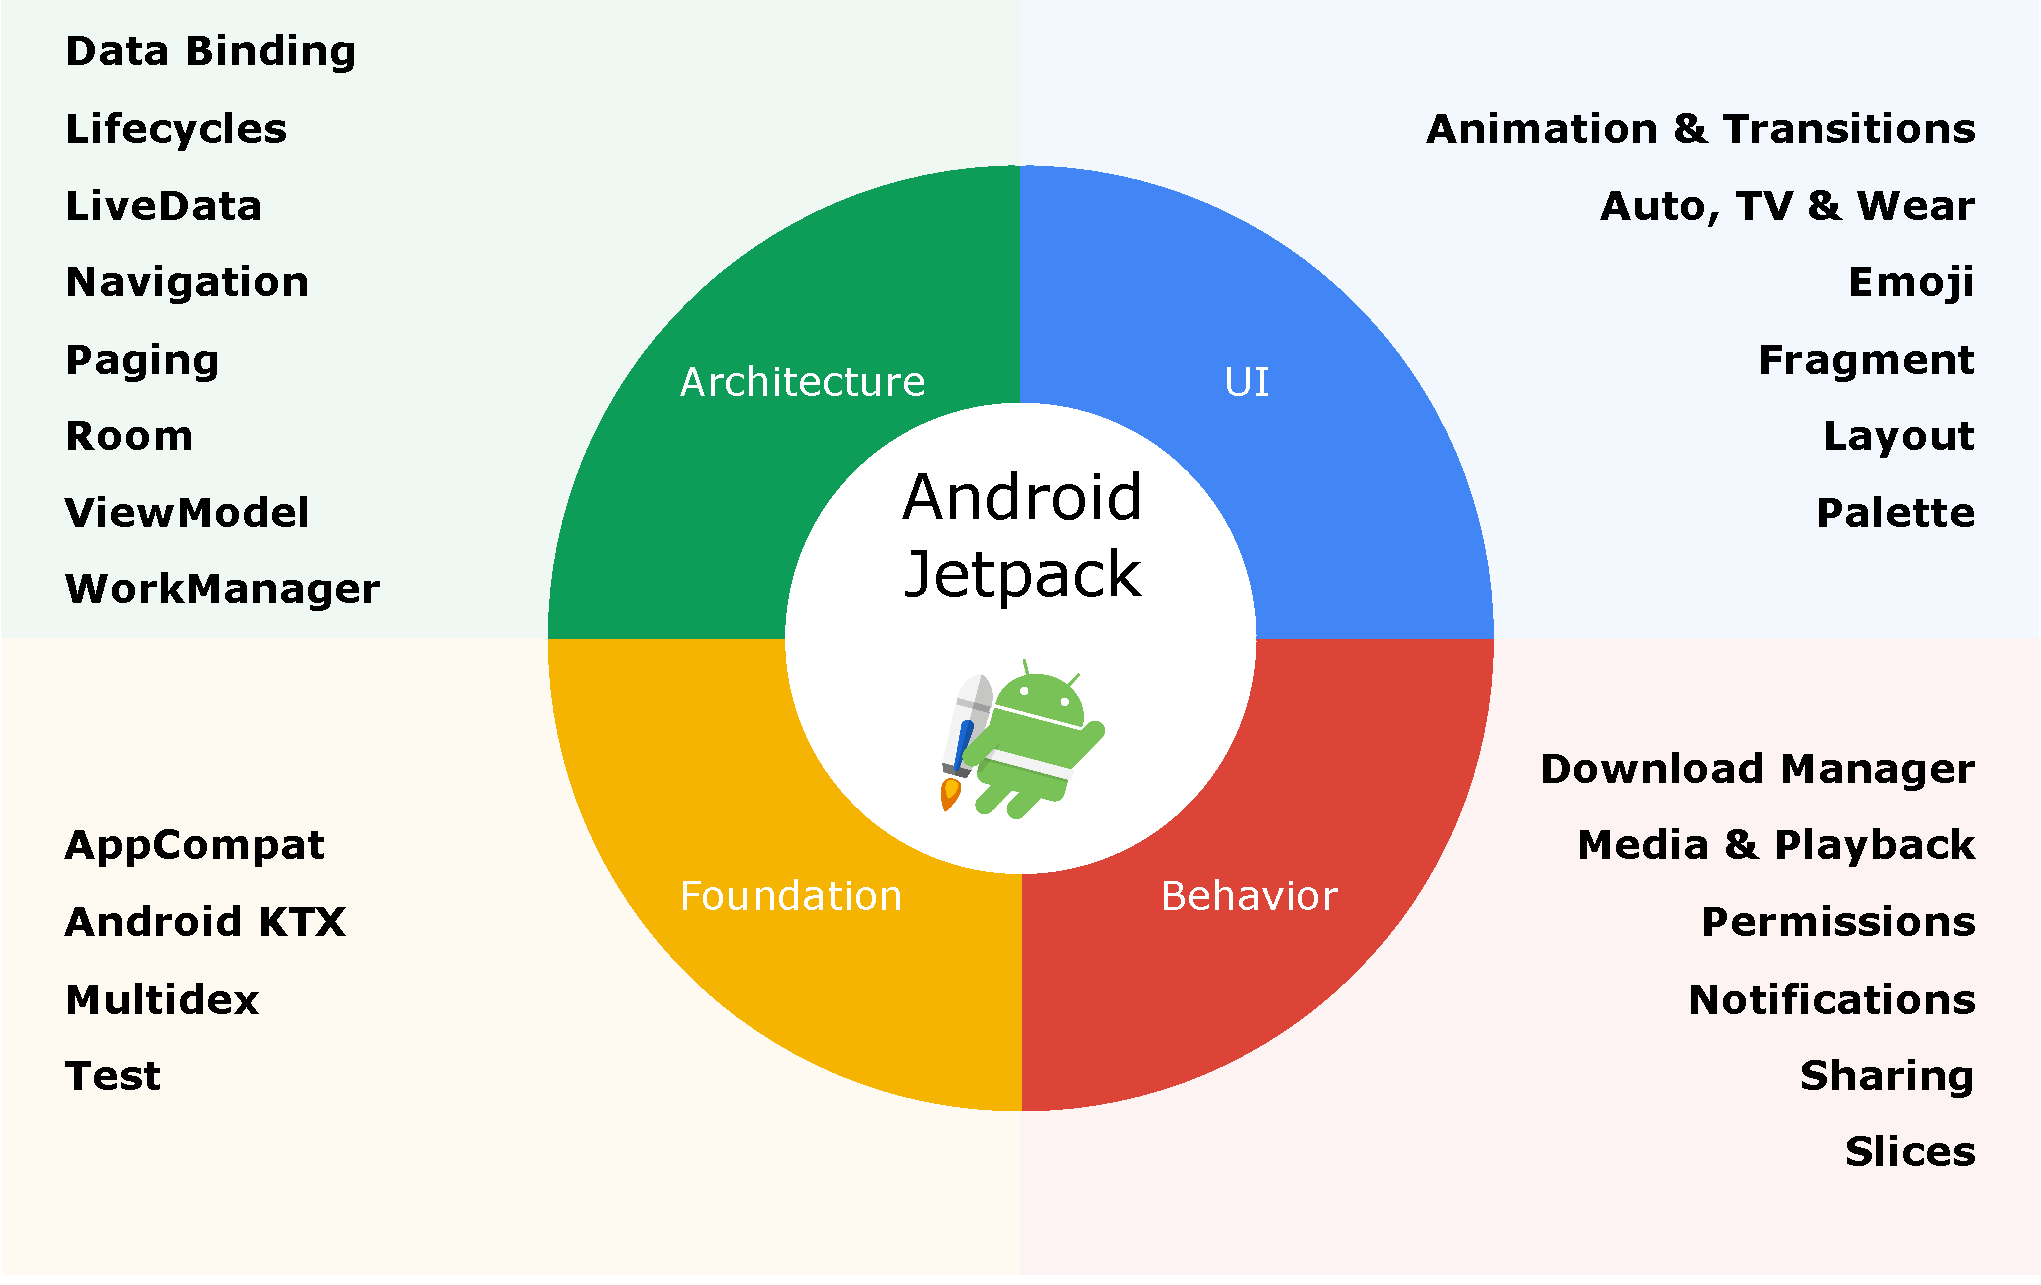
\includegraphics[width=\textwidth]{images/AndroidJetpackUebersicht.drawio.pdf}
    % \captionsetup{justification=centering}
    \caption{Überblick über die Komponenten von Android Jetpack}{Quelle: In Anlehnung an \cite{android_jetpack_ueberblick}}
    \label{fig:AndroidJetpackUebersicht}
\end{figure}

Android Jetpack ist eine Sammlung von Bibliotheken und soll Entwicklern*innen dabei helfen, Best Practices zu befolgen, Boilerplate-Code zu reduzieren und Code zu schreiben, der über alle Android-Versionen und -Geräte hinweg konsistent funktioniert \cite{android_jetpack}. Da die Komponenten so aufgebaut sind, dass ihre Funktionalität versionsunabhängig zur Verfügung steht, ist die Abwärtskompatibilität gewährleistet \cite{android_jetpack_ueberblick}. Damit haben Entwickler*innen mehr Zeit, sich auf den Code zu konzentrieren, der für ihre App wichtig ist, um leichter und schneller, robuste und hochwertige Apps zu entwickeln. 

Android Jetpack verwaltet also Aktivitäten wie Hintergrundaufgaben, Navigation und Lebenszyklusmanagement. Jetpack ist für eine gute Zusammenarbeit mit Kotlin konzipiert und zusätzlich kann mit der Komponente Android KTX einiges an Code eingespart werden. Die von Jetpack verwalteten Aktivitäten, Kotlin und die Komponenten Android KTX tragen daher gemeinsam dazu bei, den Boilerplate-Code zu eliminieren. \cite{android_whats_new}

Die Android Jetpack-Komponenten sind als sogenannte unbundled Libraries bereitgestellt und sind nicht Teil der Android-Plattform. Dadurch können Updates der Libraries auch unabhängig und öfter durchgeführt werden \cite{androidx_releases}. Diese Libraries wurden alle in den neuen \lstinline{androidx.*} Namespace verschoben und können einzeln oder auch in Kombination verwendet werden. \cite{android_jetpack_ueberblick} Daher ist AndroidX eine wesentliche Verbesserung zu der ursprünglichen Android Support Library, welche nicht mehr gewartet wird \cite{androidx_ueberblick}. 


\chapter{Android Jetpack-Komponenten}
\label{chap:androidJetpack-Komponenten}

Um mit den Android Jetpack-Komponenten zu starten, ist es wichtig zu wissen, wie diese zu einem Projekt hinzugefügt werden können. Die gesamten Jetpack-Komponenten sind im Google Maven Repository\footnote{\url{https://maven.google.com/web/index.html} Zugriff am 10.12.2022} verfügbar. \cite{android_jetpack_getting_started}

Wird in Android Studio ein neues Compose Projekt angelegt, so wird die \lstinline{settings.gradle} Datei wie in Listing \ref{lst:settings.gradle} ersichtlich automatisch angelegt.

\begin{lstlisting}[frame=lines, caption=\lstinline{settings.gradle} Datei\\Quelle: Eigenes Listing, captionpos=b, label = lst:settings.gradle, language=Groovy, showstringspaces=false]
pluginManagement {
    repositories {
        gradlePluginPortal()
        google()
        mavenCentral()
    }
}
dependencyResolutionManagement {
    repositoriesMode.set(RepositoriesMode.FAIL_ON_PROJECT_REPOS)
    repositories {
        google()
        mavenCentral()
    }
}
rootProject.name = "TestApp"
include ':app'
\end{lstlisting}

Hier ist es wichtig, dass das \lstinline{google()} Repository in dem \lstinline{repositories} Block, welcher sich im \lstinline{dependencyResolutionManagement} Block befindet, eingetragen ist, um Jetpack-Komponenten vom Google Maven Repository verwenden zu können. Anschließend ist es möglich, in der \lstinline{build.gradle} Datei im \lstinline{App} Ordner, Jetpack-Komponenten hinzuzufügen. \cite{android_jetpack_getting_started} Um zum Beispiel die CameraX Komponente hinzuzufügen, wird innerhalb des Blocks der \lstinline{dependencies} die Codezeile, die in Listing \ref{lst:androidx.camera} zu sehen ist, hinzugefügt. 

\begin{lstlisting}[frame=lines, caption=Codezeile zum Hinzufügen der CameraX Komponente\\Quelle: Eigenes Listing, captionpos=b, label = lst:androidx.camera, language=Groovy, showstringspaces=false]
implementation 'androidx.camera:camera-camera2:1.3.0-alpha02'
\end{lstlisting}

Im Listing \ref{lst:build.gradle} ist die \lstinline{build.gradle} Datei aus dem \lstinline{App} Ordner mit den Komponenten ersichtlich, die automatisch nach Anlegen des Projekts enthalten sind. Der \lstinline{android} Konfigurationsblock wurde in diesem Listing aufgrund seiner Größe nicht integriert.

\begin{lstlisting}[frame=lines, caption=\lstinline{build.gradle} Datei im \lstinline{App} Ordner\\Quelle: Eigenes Listing, captionpos=b, label = lst:build.gradle, language=Groovy, showstringspaces=false]
plugins {
    id 'com.android.application'
    id 'org.jetbrains.kotlin.android'
    id 'kotlin-kapt'
}

android {
    ...
}

dependencies {
    implementation 'androidx.core:core-ktx:1.9.0'
    implementation 'androidx.lifecycle:lifecycle-runtime-ktx:2.5.1'
    implementation 'androidx.activity:activity-compose:1.6.1'
    implementation "androidx.compose.ui:ui:$compose_ui_version"
    implementation "androidx.compose.ui:ui-tooling-preview:$compose_ui_version"
    implementation 'androidx.compose.material:material:1.3.0'
    testImplementation 'junit:junit:4.13.2'
    androidTestImplementation 'androidx.test.ext:junit:1.1.3'
    androidTestImplementation 'androidx.test.espresso:espresso-core:3.4.0'
    androidTestImplementation "androidx.compose.ui:ui-test-junit4:$compose_ui_version"
    debugImplementation "androidx.compose.ui:ui-tooling:$compose_ui_version"
    debugImplementation "androidx.compose.ui:ui-test-manifest:$compose_ui_version"
}
\end{lstlisting}

Eine gewisse Anzahl an Jetpack-Bibliotheken bieten Android KTX Erweiterungen, welche auf der Java-basierten API aufbauen und Kotlin-spezifische Sprachfunktionen nutzen \cite{android_jetpack_getting_started}. Wie schon erwähnt, werden die Jetpack-Bibliotheken im \lstinline{androidx} Namespace veröffentlicht. Nutzt ein Projekt noch die Android Support Library, dann kann diese in den \lstinline{androidx} Namespace migriert werden \cite{migrate_to_androidx}.


\section{Versionierung}

Die Versionsnummer der verschiedenen Bibliotheken besteht aus drei Zahlen und hat bei Vorabversionen zusätzlich einen Suffix, der die jeweilige Vorabversionsphase angibt. Die erste Zahl von links beginnenden repräsentiert Major, die zweite Minor und die dritte das Bugfix-Level. Bei Vorabversionen wird hinter diesen drei Zahlen entweder Alpha, Beta oder Release Candidate hinzugefügt. Wobei Alpha für eine stabile Version steht, die jedoch noch nicht alle Features inkludiert hat und Application Programming Interfaces (APIs) noch hinzugefügt, entfernt oder geändert werden können. Bei Beta-Versionen handelt es sich wieder um stabile Versionen, die auch über eine vollständige API-Oberfläche verfügen, jedoch Fehler enthalten können. Release Candidate ist eine voraussichtlich stabile Version mit einer endgültigen API-Oberfläche. Bibliotheken, die keinen Suffix besitzen, sind sogenannte Stable-Versionen, die stabil laufen und alle Funktionen implementiert haben. Eine Bibliothek kann auch mehrere Versionen gleichzeitig besitzen, wobei jede Version ein anderes Release-Stadium hat. Eine Bibliothek kann beispielsweise eine Stable, eine Alpha- und eine Beta-Version gleichzeitig besitzen. \cite{androidx_releases}


\section{Activity}

In einer Android-Anwendung sind Aktivitäten eine wesentliche Komponente. Die Art und Weise, wie Activities gestartet und zusammengestellt werden, ist ein grundlegender Teil des Anwendungsmodells der Plattform. Während in anderen Programmierstilen Apps mit einer \lstinline{main()}-Methode gestartet werden, gibt es im Android-System ein anderes Konzept für den Start von Code in der App. Android initiiert den Code in einer \lstinline{Activity}-Instanz, indem es bestimmte Callback-Methoden aufruft, die bestimmten Phasen des Lebenszyklus entsprechen. \cite{android_activities}

Die Interaktion mit einer App beginnt nicht immer an derselben Stelle, wird zum Beispiel eine E-Mail-App vom Startbildschirm aus geöffnet, dann ist meistens eine Liste von E-Mails zu sehen. Wenn jedoch eine andere App die E-Mail-App öffnet, ist möglicherweise der Bildschirm zum Verfassen einer neuen E-Mail sichtbar. Um diesen Stil zu unterstützen, wurde die \lstinline{Activity}-Klasse entwickelt. Ruft also eine App eine andere App auf, so wird eine Aktivität in der Ziel-App aufgerufen und nicht die App als Ganzes. Die Aktivität dient daher als Einstiegspunkt für diese Interaktion. Die meisten Anwendungen enthalten mehrere Screens und bestehen daher aus mehreren Aktivitäten. Üblicherweise ist der erste Screen beim Starten die Hauptaktivität. Jede Aktivität hat die Möglichkeit, eine andere Aktivität zu starten, beispielsweise kann aus dem Posteingang einer E-Mail-App ein neuer Screen für das Schreiben einer neuen E-Mail gestartet werden. Trotz der Zusammenarbeit von Aktivitäten besteht in einer App nur eine minimale Abhängigkeit zwischen ihnen. Um Aktivitäten verwenden zu können, müssen Informationen über sie im Manifest der App registriert werden und auch die Lebenszyklen der Aktivitäten verwaltet werden. \cite{android_activities} Seit 2018 geht der Trend für die Strukturierung der In-App Bedienoberfläche, durch die Einführung der Android Jetpack-Komponente Navigation, zur Single-Activity-App Architektur \cite{android_jetpack_ueberblick}.


\section{Lifecycle}

Wenn eine*ein Benutzer*in innerhalb, aus und zurück in die App navigiert, wechseln die Zustände der Aktivität in ihrem Lebenszyklus. Die \lstinline{Activity}-Klasse bietet verschiedene Callbacks, die der Aktivität mitteilen, dass sich der Zustand verändert hat. Mit den Lifecycle-Callback-Methoden können Entwickler*innen bestimmen, wie sich die Aktivität verhalten soll, wenn die App verlassen wird und später wieder aufgerufen wird. Das heißt, jeder Callback kann bestimmte Aufgaben ausführen, die für einen bestimmten Zustandswechsel passend sind. Die korrekte Implementierung der Lifecycle-Callbacks verbessert die Robustheit, Leistungsfähigkeit und verhindert unerwünschtes Verhalten der App. Durch diese korrekte Implementierung können folgende Beispiele, wie in „The activity lifecycle“ beschrieben, vermieden werden. \cite{android_lifecycle}

\begin{itemize} 
  \item Absturz der App, wenn bei der Verwendung der App ein Anruf eintrifft oder während der Verwendung zu einer anderen App gewechselt wird.
  \item Verbrauch wertvoller Systemressourcen, wenn die App nicht aktiv verwendet wird.
  \item Der Verlust des Fortschritts, wenn die App verlassen wird und zu einem späteren Zeitpunkt wieder aufgerufen wird.
  \item Absturz oder Verlust des Fortschritts, wenn zwischen Hoch- und Querformat gewechselt wird.
\end{itemize}

Um die Übergänge zwischen den einzelnen Phasen des Aktivitätslebenszyklus zu steuern, stellt die \lstinline{Activity}-Klasse ein Set von sieben Callbacks zur Verfügung. Das System ruft diese Callbacks auf, sobald eine Aktivität einen neuen Zustand erreicht. \cite{android_lifecycle} Die einzelnen Callbacks mit ihren grundlegenden Funktionen sind hier, wie im Abschnitt "Activity Lifecycle", angeführt \cite{android_activity}.

\begin{itemize} 
  \item \textbf{\lstinline{onCreate()}} \\ 
        Wird aufgerufen, wenn die Aktivität zum ersten Mal erstellt wird. \\
        Es folgt immer \lstinline{onStart()}.
  \item \textbf{\lstinline{onRestart()}} \\ 
        Diese Callback-Methode wird aufgerufen, nachdem die Aktivität gestoppt wurde und bevor sie wieder gestartet wird. \\
        Es folgt immer \lstinline{onStart()}.
  \item \textbf{\lstinline{onStart()}} \\ 
        Der Aufruf erfolgt, wenn die Aktivität für die*den Benutzer*in sichtbar wird. \\
        Es folgt immer \lstinline{onResume()}.
  \item \textbf{\lstinline{onResume()}} \\ 
        Wird aufgerufen, wenn die Aktivität beginnt, mit der*dem Benutzer*in zu interagieren und Eingaben gehen direkt an die Aktivität. \\
        Es folgt immer \lstinline{onPause()}.
  \item \textbf{\lstinline{onPause()}} \\ 
        Der Aufruf von \lstinline{onPause()} erfolgt, wenn die Aktivität den Vordergrundstatus verliert, nicht mehr fokussierbar ist oder vor dem Übergang in den Zustand \lstinline{onStop()} oder \lstinline{onDestroy()}. \\
        Wenn die Aktivität wieder in den Vordergrund tritt, folgt \lstinline{onResume()} oder \lstinline{onStop()}, wenn sie für die*den Benutzer*in nicht mehr sichtbar ist. 
  \item \textbf{\lstinline{onStop()}} \\ 
        Dieser Callback wird aufgerufen, wenn die Aktivität für die*den Benutzer*in nicht mehr sichtbar ist. Das passiert, wenn eine neue Aktivität gestartet wird, beziehungsweise eine andere Aktivität vor dieses geschoben wird oder diese Aktivität zerstört wird. \\
        Es folgt entweder \lstinline{onRestart()}, wenn die Aktivität zurückkehrt, um damit wieder zu interagieren oder \lstinline{onDestroy()}, wenn die Aktivität verschwindet. 
  \item \textbf{\lstinline{onDestroy()}} \\ 
        Ist der letzte Callback, bevor die Aktivität zerstört wird, entweder weil die Aktivität durch \lstinline{finish()} beendet wird oder weil das System diese Instanz der Aktivität vorübergehend zerstört, um Platz zu sparen.\\
        Nach diesem Callback folgen keine anderen Callbacks mehr.
\end{itemize}

Abbildung \ref{fig:Aktivitätslebenszyklus} zeigt die verschiedenen Callbacks in einem vereinfachten Aktivitätslebenszyklus. 

\begin{figure}[H]
	\centering
		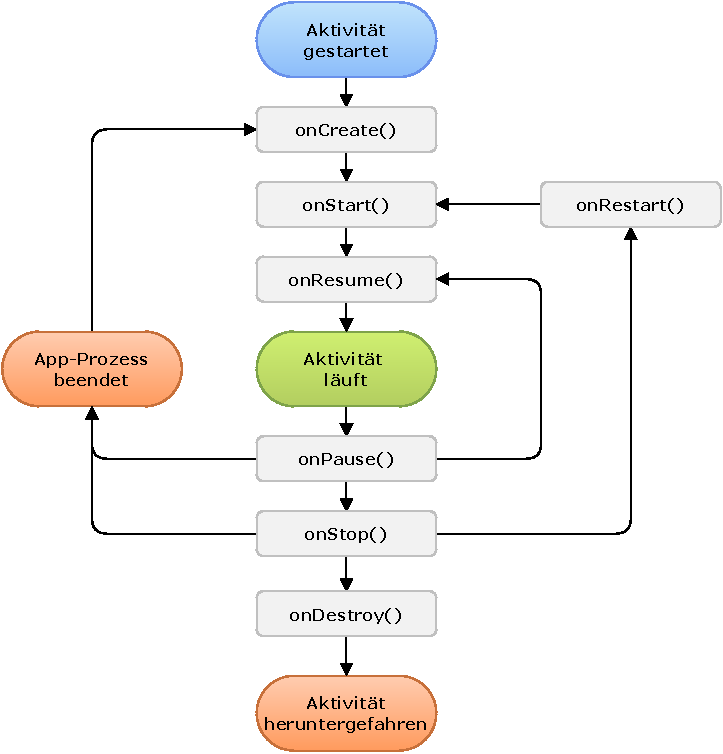
\includegraphics[]{images/Aktivitaetslebenszyklus.drawio.pdf}
	\caption{Callbacks im Aktivitätslebenszyklus}{Quelle: In Anlehnung an \cite{android_lifecycle}}
	\label{fig:Aktivitätslebenszyklus}
\end{figure}

Das \lstinline{androidx.lifecycle}-Paket bietet Klassen und Schnittstellen an, mit denen Komponenten erstellt werden können, die den Lebenszyklus einer Aktivität oder eines Fragments berücksichtigen und ihr Verhalten automatisch an diesen Lebenszyklus anpassen. Diese sogenannten Lifecycle-Aware Components führen, aufgrund einer Änderung des Lebenszyklus einer anderen Aktivität, Aktionen aus. \cite{android_architecture_lifecycle}

Die \lstinline{Lifecycle}-Klasse enthält Informationen über den Zustand des Lebenszyklus einer Komponente und ermöglicht anderen Objekten, diesen Zustand zu beobachten. Um den Lebenszyklus für eine zugehörige Komponente zu verfolgen, verwendet die \lstinline{Lifecycle}-Klasse verschiedene Ereignisse und Zustände. Einerseits die Ereignisse oder Events, die vom Framework und der \lstinline{Lifecycle}-Klasse ausgeführt werden und den Callback-Ereignissen in den Aktivitäten entsprechen und andererseits den aktuellen Zustand, der vom \lstinline{Lifecycle}-Objekt verfolgt wird. \cite{android_architecture_lifecycle}

\lstinline{LifecycleOwner} ist eine Schnittstelle, die eine Methode hat und angibt, dass eine Klasse einen Lebenszyklus hat. Die Methode \lstinline{getLifecycle()} muss von der Klasse implementiert werden. Jede individuell definierte Klasse kann die \lstinline{LifecycleOwner}-Schnittstelle implementieren. Fragmente und Aktivitäten im \lstinline{androidx} Namespace implementieren bereits die \lstinline{LifecycleOwner}-Schnittstelle. Komponenten, die \lstinline{DefaultLifecycleObserver} implementiert haben, arbeiten mit Komponenten, die \lstinline{LifecycleOwner} implementiert haben zusammen, weil ein Owner seinen Lebenszyklus zur Beobachtung freigibt und sich ein Observer zur Beobachtung anmelden kann. \cite{android_architecture_lifecycle} Der \lstinline{DefaultLifecycleObserver} ist also eine sogenannte Callback-Schnittstelle zum Abhören von \lstinline{LifecycleOwner} Zustandsänderungen \cite{DefaultLifecycleObserver}.

Im Listing \ref{lst:LifecycleObserverUndLifecycleOwner} ist die Klasse \lstinline{MyObserver}, die das Interface \lstinline{DefaultLifecycleObserver} implementiert, um den Lebenszyklusstatus des \lstinline{LifecycleOwners} zu überwachen und die beiden Methoden \lstinline{onResume} und \lstinline{onPause} überschreibt, zu sehen. Zusätzlich wird über das Objekt \lstinline{myLifecycleOwner}, welches die Schnittstelle \lstinline{LifecycleOwners} implementiert, ein Observer hinzugefügt, indem die Methode \lstinline{addObserver()} der \lstinline{Lifecycle}-Klasse aufgerufen wird und eine Instanz des \lstinline{Observers} übergeben wird \cite{android_architecture_lifecycle}.

\begin{lstlisting}[frame=lines, caption=Beispeilcode für \lstinline{LifecycleObserver} und \lstinline{LifecycleOwner}\\Quelle: \cite{android_architecture_lifecycle}, captionpos=b, label = lst:LifecycleObserverUndLifecycleOwner, language=Kotlin, showstringspaces=false]
class MyObserver : DefaultLifecycleObserver {
    override fun onResume(owner: LifecycleOwner) {
        connect()
    }

    override fun onPause(owner: LifecycleOwner) {
        disconnect()
    }
}

myLifecycleOwner.getLifecycle().addObserver(MyObserver())
\end{lstlisting}

Einige Anwendungsfälle für die Verwendung von Lifecycle-Aware Components, die in „Use cases for lifecycle-aware components“ beschrieben sind zum Beispiel: \cite{android_architecture_lifecycle}
\begin{itemize}
  \item Umschalten zwischen grob- und feinkörnigen Standortaktualisierungen.
  \item Anhalten und Starten der Videopufferung.
  \item Starten und Stoppen der Netzwerkverbindung.
  \item Anhalten und Fortsetzen von animierten Zeichenflächen.
\end{itemize}


\subsection{ViewModel}

Die Klasse \lstinline{ViewModel} hält den Status für die Geschäftslogik oder die Bildschirmebene, sie stellt den Zustand der Benutzungsoberfläche zur Verfügung und kapselt die Geschäftslogik \cite{viewmodel_overview}. Ein \lstinline{ViewModel} ist für die Vorbereitung und Verwaltung der Daten für eine Aktivität oder ein Fragment verantwortlich und übernimmt auch die Kommunikation zwischen Aktivität und Fragment mit dem Rest der Anwendung \cite{viewmodel}. Der Hauptvorteil der Arbeitsweise von \lstinline{ViewModel} ist, dass der Status zwischengespeichert wird und auch bei Konfigurationsänderungen beibehalten wird. Die Bedienoberfläche muss daher die Daten nicht erneut abrufen, wenn zwischen Aktivitäten navigiert wird. Dabei handelt es sich zum Beispiel um das Drehen des Bildschirms. \cite{viewmodel_overview}

Eine Alternative dazu wäre eine einfache Klasse, die alle Daten der Benutzungsoberfläche enthält, wenn jedoch zwischen den Aktivitäten navigiert wird, kann es zu einem Datenverlust kommen. Um dieses Problem zu beheben, bietet \lstinline{ViewModel} eine API, welche auch für Datenpersistenz sorgt. \cite{viewmodel_overview}

Einem \lstinline{ViewModel}, das instanziiert wird, wird ein Objekt übergeben, das die Schnittstelle \lstinline{ViewModelStoreOwner} implementiert. Das \lstinline{ViewModel} wird anschließend in den Lebenszyklus des \lstinline{ViewModelStoreOwner} integriert und bleibt so lange im Speicher, bis sein \lstinline{ViewModelStoreOwner} dauerhaft verschwindet. Dies kann in den folgenden Fällen auftreten, wie in „The lifecycle of a ViewModel“ erwähnt. \cite{viewmodel_overview}

\begin{itemize}
  \item Im Falle einer Aktivität, wenn sie beendet ist.
  \item Im Falle eines Fragments, wenn es sich loslöst.
  \item Im Falle eines Navigationseintrags, wenn er aus dem Backstack entfernt wird.
\end{itemize}

Abbildung \ref{fig:ViewModelLebenszyklus} zeigt sowohl die unterschiedlichen Zustände vom Lebenszyklus einer Aktivität als auch die Lebensdauer des \lstinline{ViewModels}, während die Aktivität eine Rotation durchläuft und dann beendet wird. Dabei existiert das \lstinline{ViewModel} von der ersten Anforderung bis zur Beendigung und Zerstörung der Aktivität. \cite{viewmodel_overview}

\begin{figure}[H]
	\centering
		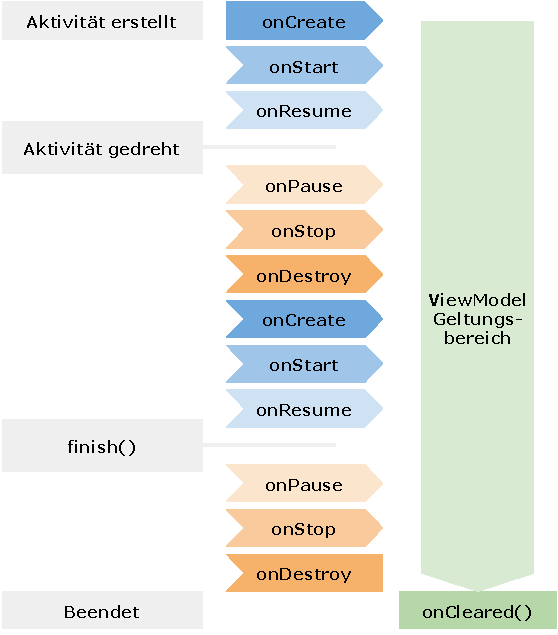
\includegraphics[]{images/ViewModelLifecycle.drawio.pdf}
	\caption{Lebenszyklus eines \lstinline{ViewModels}}{Quelle: In Anlehnung an \cite{viewmodel_overview}}
	\label{fig:ViewModelLebenszyklus}
\end{figure}

Die Schnittstelle \lstinline{ViewModelStoreOwner} besitzt eine Reihe von direkten oder indirekten Unterklassen. Bei \lstinline{ComponentActivity}, \lstinline{Fragment} und \lstinline{NavBackStackEntry} handelt es sich um direkte Unterklassen. \cite{viewmodel_overview}

Die asynchrone Arbeit im \lstinline{ViewModel} wird auch fortgesetzt, wenn ein Fragment oder eine Aktivität, auf die das \lstinline{ViewModel} skaliert ist, zerstört wird \cite{viewmodel_overview}.

Da die UI-Schicht in bestimmten Fällen auch Geschäftslogik enthalten kann, ist das \lstinline{ViewModel} geeignet, diese zu behandeln. Muss Geschäftslogik zur Änderung von Daten angewendet werden, ist das \lstinline{ViewModel} auch für diese Bearbeitung von Ereignissen zuständig. \cite{viewmodel_overview}

\subsection{LiveData}

Die Informationen, die das ViewModel für eine Aktivität oder ein Fragment speichert, können vom ViewModel über LiveData zur Verfügung gestellt werden. \lstinline{LiveData} ist eine Klasse, die beobachtbar ist und Daten hält. LiveData ist dabei lebenszyklusorientiert und berücksichtigt den Lebenszyklus von Aktivitäten und Fragmenten nur dann, wenn sich diese auch in einem aktiven Lebenszyklus-Zustand befinden. \cite{livedata_overview}

LiveData nimmt zu einem Observer, der durch die Klasse \lstinline{Observer} repräsentiert wird, nur Verbindung auf, wenn dieser in einem aktiven Zustand ist, also sein Lebenszyklus sich im Zustand \lstinline{STARTED} oder \lstinline{RESUMED} befindet. Inaktive Observer werden jedoch nicht über Updates informiert. \cite{livedata_overview}

Ein Observer kann mit einem Objekt registriert werden, das die Schnittstelle \lstinline{LifecycleOwner} implementiert. Dadurch wird der Observer auch wieder sofort entfernt, wenn das entsprechende \lstinline{Lifecycle}-Objekt in den Status \lstinline{DESTROYED} wechselt. Für Aktivitäten und Fragmente ist das besonders nützlich, weil \lstinline{LiveData}-Objekte sicher beobachtet werden und keine Lecks entstehen. Die Verwendung von LiveData hat folgende Vorteile, wie im Abschnitt „The advantages of using LiveData“ angeführt. \cite{livedata_overview}

\begin{itemize} 
  \item \textbf{Sicherstellung, der Übereinstimmung von Bedienoberfläche und Datenzustand} \\ 
        Die Benutzungsoberfläche muss nicht jedes Mal aktualisiert werden, wenn sich Anwendungsdaten ändern, denn diesen Vorgang übernimmt der Observer. 
  \item \textbf{Keine Speicherlecks} \\ 
        Observer sind an \lstinline{Lifecycle}-Objekte gebunden und geben ihre Ressourcen frei, wenn ihr zugehöriger Lifecycle zerstört wird.
  \item \textbf{Keine Abstürze aufgrund von gestoppten Aktivitäten} \\ 
        Wenn der Lebenszyklus des Observers inaktiv ist, beispielsweise wenn sich die Aktivität im Backstack befindet, dann erhält er keine LiveData-Ereignisse.
  \item \textbf{Keine manuelle Verwaltung des Lebenszyklus mehr} \\ 
        UI-Komponenten beobachten nur relevanten Daten und die Beobachtung wird weder gestoppt noch fortgesetzt. LiveData verwaltet alles automatisch, da die relevanten Änderungen des Lebenszyklusstatus während der Beobachtung bekannt sind.
  \item \textbf{Immer aktuelle Daten} \\ 
        Ein Lebenszyklus, der inaktiv wird, erhält die neuesten Daten, sobald er wieder aktiv wird.
  \item \textbf{Ordnungsgemäße Konfigurationsänderungen} \\ 
        Wird eine Aktivität oder ein Fragment aufgrund einer Konfigurationsänderung, wie zum Beispiel der Bildschirmdrehung neu erstellt, erhält es sofort die aktuellsten verfügbaren Daten.
  \item \textbf{Gemeinsame Nutzung von Ressourcen} \\ 
        Mit dem Singleton Pattern kann ein \lstinline{LiveData}-Objekt erweitert werden, um Systemdienste so zu verpacken, dass sie in der Anwendung gemeinsam genutzt werden können. Das \lstinline{LiveData}-Objekt verbindet sich einmal mit dem Systemdienst und jeder Observer, der die Ressource benötigt, kann das Objekt beobachten. 
\end{itemize}


\section{Paging}

Beim Arbeiten mit größeren Datensätzen, die aus dem lokalen Speicher oder über das Netzwerk geladen und anschließend angezeigt werden, ist der Einsatz der Paging-Bibliothek hilfreich. Paging ermöglicht es Netzwerkbandbreite, aber auch Systemressourcen effizienter zu nutzen. Die Komponenten der Paging-Bibliothek lassen sich problemlos mit anderen Jetpack-Komponenten kombinieren und bieten Kotlin-Support. \cite{paging_overview}

Die Paging-Bibliothek enthält die folgenden Funktionen, wie in „Benefits of using the Paging library“ beschrieben \cite{paging_overview}.

\begin{itemize} 
  \item Durch In-Memory-Caching wird sichergestellt, dass die Anwendung bei der Arbeit mit ausgelagerten Daten die Systemressourcen effizient nutzt.
  \item Effiziente Nutzung der Netzwerkbandbreite und Systemressourcen durch integrierte Anforderungs-Deduplizierung.
  \item Konfigurierbare \lstinline{RecyclerView}-Adapter, die automatisch Daten anfordern, wenn die*der Benutzer*in zum Ende der geladenen Daten scrollt.
  \item Unterstützt Kotlin Coroutines und Flow sowie LiveData und RxJava.
  \item Integrierte Unterstützung für die Fehlerbehandlung, inklusive Aktualisierungs- und Wiederholungsfunktionen.
\end{itemize}

Die Paging-Bibliothek ist in die Android-App-Architektur direkt integrierbar, wobei die Komponenten der Bibliothek in einer App in drei Schichten arbeiten. Bei den drei Schichten handelt es sich um die Repository-Schicht, die ViewModel-Schicht und die UI-Schicht, wie auch in Abbildung \ref{fig:PagingBibliothekArchitektur} ersichtlich ist. \cite{paging_overview}

\begin{figure}[H]
	\centering
		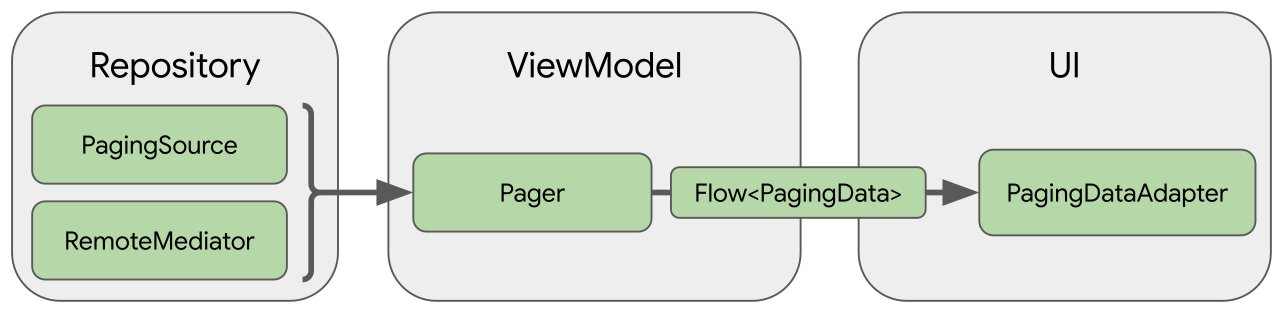
\includegraphics[width=\textwidth]{images/PagingBibliothekArchitektur.jpg}
	\caption{Architektur der Paging-Bibliothek}{Quelle: \cite{paging_overview}}
	\label{fig:PagingBibliothekArchitektur}
\end{figure}

\noindent\textbf{Repository-Schicht} \\
Die wichtigste Komponente in der Repository-Schicht ist \lstinline{PagingSource}. Ein \lstinline{PagingSource}-Objekt legt eine Datenquelle fest und definiert, wie die Daten aus dieser Quelle abgerufen werden. \cite{paging_overview}

Eine weitere Komponente ist der \lstinline{RemoteMediator}, welcher das Paging aus einer mehrschichtigen Datenquelle, zum Beispiel eine Netzwerkdatenquelle mit einem lokalen Datenbank-Cache verwaltet \cite{paging_overview}. 

\noindent\textbf{ViewModel-Schicht} \\
Die \lstinline{Pager} Komponente bietet eine öffentliche API zur Erstellung von Instanzen von \lstinline{PagingData}, die in reaktiven Streams auf der Grundlage eines \lstinline{PagingSource}-Objekts und eines \lstinline{PagingConfig}-Konfigurationsobjekts dargestellt werden \cite{paging_overview}.

\lstinline{PagingData} ist eine Komponente, welche die \lstinline{ViewModel}-Schicht mit der Bedienoberfläche verbindet. Ein \lstinline{PagingData}-Objekt fragt ein \lstinline{PagingSource}-Objekt ab und speichert das Ergebnis \cite{paging_overview}. 

\noindent\textbf{UI-Schicht} \\
Der \lstinline{PagingDataAdapter} in der UI-Schicht ist ein RecyclerView-Adapter, der die Paging Daten verarbeitet. Bei Verwendung von Jetpack Compose für das UI wird \lstinline{collectAsLazyPagingItems()} verwendet, um die Daten entweder in einer Lazy list oder in einem Lazy grid anzuzeigen. \cite{paging_overview}


\section{DataStore}

Bei der DataStore-Bibliothek handelt es sich um eine neue und verbesserte Datenspeicherlösung, welche die SharedPreferences ersetzen soll, dabei werden die Daten unter Verwendung von Kotlin Coroutines und Flow asynchron, konsistent und transaktional gespeichert. Dadurch werden die meisten Nachteile von SharedPreferences beseitigt. \cite{datastore_releases}

Mit der DataStore-Bibliothek sind zwei verschiedene Implementierungen möglich. Bei der ersten Implementierung, \mbox{Preferences DataStore} werden Daten mithilfe von Schlüsseln gespeichert und auf sie zugegriffen, wobei kein vordefiniertes Schema verwendet werden muss und es keine Typensicherheit bietet. Die zweite Implementierung ist \mbox{Proto DataStore}, bei dieser werden die Daten als Instanzen eines individuell definierten Datentyps gespeichert. Diese Art der Implementierung benötigt die Definition eines Schemas unter Verwendung von Protokollpuffern, dafür wird jedoch Typsicherheit geboten. \cite{datastore}

DataStore eignet sich für kleine, einfache Datensätze und es ist darauf zu achten, dass es keine partiellen Aktualisierungen oder referenzielle Integrität unterstützt. Wird mit großen oder komplexen Datensätzen gearbeitet, partielle Aktualisierungen oder referenzielle Integrität benötigt, dann sollte Room anstelle von DataStore verwendet werden. \cite{datastore}


\section{Room}

Bei Room handelt es sich um eine Database Object Mapping Bibliothek, die den Datenbankzugriff in Android-Anwendungen erleichtert. Room stellt APIs zur Abfrage der Datenbank und zur Überprüfung dieser Abfragen während der Kompilierungszeit zur Verfügung. \cite{androidx.room} Room stellt eine Schicht zwischen Anwendung und SQLite bereit, die es ermöglicht, auf die Datenbank zuzugreifen, ohne sich um die Details der SQLite-Implementation kümmern zu müssen, während dennoch die volle Leistung von SQLite und die Typsicherheit von Java und Kotlin SQL Query Buildern genutzt werden kann \cite{androidx.room}, \cite{room}. Außerdem bietet Room optimierte Migrationspfade für Datenbanken und Annotationen, die wiederholenden und fehleranfälligen Boilerplate-Code minimieren. Aufgrund der Vorteile, die diese Bibliothek bietet, wird empfohlen Room zu verwenden, anstatt die SQLite-APIs direkt zu nutzen. \cite{room}

Die drei wichtigsten Komponenten von Room sind die Room Datenbank, Data Access Objects (DAOs) und Entities, deren Beziehungen untereinander in Abbildung \ref{fig:RoomArchitektur} zu sehen sind. Die Datenbank stellt der Anwendung Instanzen der DAOs zur Verfügung, welche mit der Datenbank verknüpft sind und die App kann diese DAOs verwenden, um Daten aus der Datenbank als Instanzen der zugehörigen Data Entity Objects abzurufen. Außerdem kann die Anwendung die definierten Daten-Entities verwenden, um Zeilen aus den entsprechenden Tabellen zu aktualisieren, einzufügen oder zu löschen. \cite{room}

\begin{figure}[H]
	\centering
		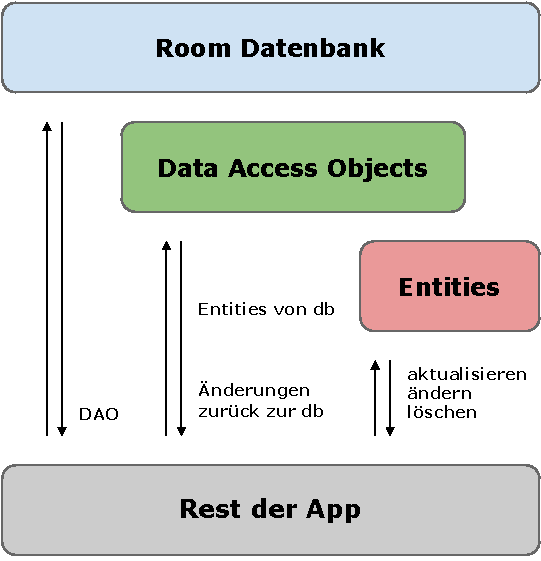
\includegraphics[]{images/RoomArchitektur.drawio.pdf}
	\caption{Architektur der Room-Bibliothek}{Quelle: In Anlehnung an \cite{room}}
	\label{fig:RoomArchitektur}
\end{figure}

\noindent\textbf{Data Entity} \\
Entities werden definiert, um Objekte darzustellen, die gespeichert werden sollen. Dabei entspricht jede Entity einer Tabelle in der Datenbank und jede Instanz stellt eine Datenzeile dar. Der Vorteil bei der Verwendung von Room-Entities ist, dass ein Datenbankschema definierbar ist, ohne SQL-Code schreiben zu müssen. \cite{room_entities} 

Jede Room-Entitiy ist eine Klasse, die mit \lstinline{@Entity} annotiert ist und enthält Felder für jede Spalte in der entsprechenden Tabelle. Eine Room-Entitiy muss einen Primärschlüssel haben. Eine oder mehre Spalten können dabei mit \lstinline{@PrimaryKey} gekennzeichnet werden, welche dann den Primärschlüssel bilden. Das Listing \ref{lst:EntityCode} zeigt eine einfache Room-Entitiy, die eine Tabelle User mit den Spalten ID, Vorname und Nachname definiert, wobei die Spalte ID der Primärschlüssel ist. \cite{room_entities}

\begin{lstlisting}[frame=lines, caption=Code einer Room-Entitiy\\Quelle: \cite{room_entities}, captionpos=b, label = lst:EntityCode, language=Kotlin, showstringspaces=false]
@Entity
data class User(
    @PrimaryKey val id: Int,
    val firstName: String?,
    val lastName: String?
)
\end{lstlisting}

\noindent\textbf{DAO} \\
In der Anwendung werden zum Speichern der Daten DAOs definiert, wobei jedes DAO Methoden enthält, die einen abstrakten Zugriff auf die Datenbank der App ermöglichen. DAOs erleichtern das Simulieren von Datenbankzugriffen beim Testen der App. \cite{room_daos}

Ein DAO kann als Schnittstelle oder abstrakte Klasse definiert werden, wobei normalerweise Schnittstellen verwendet werden. DAOs werden immer mit \lstinline{@Dao} annotiert. Um Datenbankinteraktionen zu definieren, gibt es zwei verschiedene Arten von DAO-Methoden. Einerseits die Convenience-Methoden, welche das Einfügen, Aktualisieren und Löschen von Zeilen in der Datenbank ermöglichen, ohne SQL-Code zu schreiben. Andererseits die Query-Methoden, mit denen durch eigene SQL-Anweisungen Daten aus der Datenbank abgefragt werden können oder komplexere Einfügungen, Aktualisierungen und Löschungen durchgeführt werden können und sie dabei als DAO-Methoden darzustellen. Das Listing \ref{lst:DaoCode} zeigt ein einfaches DAO als \lstinline{UserDao}-Schnittstelle, welche sowohl die Convenience-Methoden \lstinline{@Insert} und \lstinline{@Delete} als auch eine Query-Methode, die mittels eigenem SQL-Code alle User*innen aus der Datenbank abruft, beinhaltet. \cite{room_daos}

\begin{lstlisting}[frame=lines, caption=Code eines DAOs\\Quelle: \cite{room_daos}, captionpos=b, label = lst:DaoCode, language=Kotlin, showstringspaces=false]
@Dao
interface UserDao {
    @Insert
    fun insertAll(vararg users: User)

    @Delete
    fun delete(user: User)

    @Query("SELECT * FROM user")
    fun getAll(): List<User>
}
\end{lstlisting}

\noindent\textbf{Datenbank} \\
Die Datenbankklasse enthält die Datenbank, welche als Hauptzugriffspunkt für die Verbindung zu den persistierten Daten in der App dient. Diese Klasse muss eine abstrakte Klasse sein, die \lstinline{RoomDatabase} erweitert und eine \lstinline{@Database}-Annotation haben, welche ein Entity-Array enthält, das alle Data Entities auflistet, die mit der Datenbank verbunden sind. Die Datenbankklasse muss für jede DAO-Klasse, die mit der Datenbank verbunden ist, eine abstrakte Methode definieren, die keine Argumente hat und eine Instanz der DAO-Klasse zurückgibt. Im Listing \ref{lst:DatenbankCode} ist die abstrakte Klasse \lstinline{AppDatabase}, welche die \lstinline{RoomDatabase}-Klasse erweitert, mit \lstinline{@Database} annotiert ist und eine abstrakte Methode für das \lstinline{UserDao} definiert, zu sehen. \cite{room}

\begin{lstlisting}[frame=lines, caption=Code der Room Datenbank\\Quelle: \cite{room}, captionpos=b, label = lst:DatenbankCode, language=Kotlin, showstringspaces=false]
@Database(entities = [User::class], version = 1)
abstract class AppDatabase : RoomDatabase() {
    abstract fun userDao(): UserDao
}
\end{lstlisting}


\section{WorkManager}

Android fand, bei der Untersuchung der wichtigsten Probleme der Entwickler*innen, heraus, dass zuverlässige und akkuschonende Verarbeitung im Hintergrund eine große Herausforderung darstellt. Zusätzlich haben die verschiedenen Android-Versionen unterschiedliche Tools für Arbeiten im Hintergrund angeboten. Die Netzwerk- oder Speicherverfügbarkeit abzuhören und das automatische Wiederholen von Aufgaben war zum Beispiel mit viel Arbeit verbunden. \cite{workmanager_stable_release}

WorkManager erleichtert die Arbeit im Hintergrund und berücksichtigt Einschränkungen wie Akku-Optimierung, Speicherplatz oder Netzwerkverfügbarkeit. Der WorkManager führt diese Aufgaben nur aus, sofern die jeweiligen Bedingungen erfüllt sind. \cite{workmanager_stable_release} Die WorkManager-API stellt eine verbesserte Alternative für die Verwaltung von Hintergrundaufgaben in Android dar und löst damit alle früheren APIs in diesem Bereich ab, wie beispielsweise \mbox{FirebaseJobDispatcher}, \mbox{GcmNetworkManager} und \mbox{Job Scheduler} \cite{workmanager}. 

Laut Android werden die meisten Hintergrundverarbeitungen am besten durch persistente Arbeit erreicht, die auch nach einem Neustart der Anwendung oder des Systems geplant bleibt. WorkManager wird als Lösung für Hintergrundverarbeitung und daher auch für persistente Arbeit empfohlen. \cite{workmanager}

Folgende drei Arten von persistenter Arbeit kann der WorkManager verwalten, wie in „Types of persistent work“ angeführt. \cite{workmanager}

\begin{itemize} 
  \item \textbf{Immediate} \\ 
        Das sind Aufgaben, die sofort beginnen und zeitnah abgeschlossen werden müssen und auch beschleunigt werden können. Diese Aufgaben laufen einmalig. 
  \item \textbf{Long Running} \\ 
        Hierbei handelt es sich um Aufgaben, die länger dauern können, möglicherweise länger als zehn Minuten und einmalig oder periodisch ablaufen können. 
  \item \textbf{Deferrable} \\ 
        Dies sind geplante Aufgaben, die zu einem späteren Zeitpunkt beginnen und einmalig oder periodisch ausgeführt werden können. 
\end{itemize}

Neben der einfacheren und einheitlicheren API bietet der WorkManager auch eine Reihe weiterer Vorteile \cite{workmanager}. 

\noindent\textbf{Arbeitsbeschränkungen} \\
Mithilfe von Arbeitseinschränkungen ist es möglich, die Bedingungen für die Ausführung der Arbeit zu definieren. Die Arbeit soll zum Beispiel nur ausgeführt werden, wenn sich das Gerät in einem Netzwerk befindet, das nicht gebührenpflichtig ist, wenn sich das Gerät im Leerlauf befindet oder wenn der Akku ausreichend geladen ist. \cite{workmanager}

\noindent\textbf{Robuste Planung} \\
Einmalige oder wiederkehrende Arbeiten können mit WorkManager flexible geplant, gekennzeichnet und benannt werden, sodass austauschbare Arbeiten entstehen. Diese Arbeiten werden in einer internen verwalteten SQLite-Datenbank gespeichert und bleiben durch den WorkManager auch nach einem Neustart des Geräts erhalten. Zusätzlich hält sich der WorkManager an Energiesparfunktionen und bewährte Verfahren wie den Doze-Modus. \cite{workmanager}

\noindent\textbf{Beschleunigte Arbeit} \\
Sofortige Arbeiten können mit WorkManager zur Ausführung im Hintergrund geplant werden. Beschleunigte Arbeit wird innerhalb weniger Minuten abgeschlossen und sollte für Aufgaben verwendet werden, die für die*den Benutzer*in wichtig sind. \cite{workmanager}

\noindent\textbf{Flexible Wiederholungsregelungen} \\
Wenn die Arbeit fehlschlägt, bietet WorkManager flexible Wiederholungsrichtlinien inklusive einer konfigurierbaren exponentiellen Backoff-Richtline \cite{workmanager}. 

\noindent\textbf{Arbeitsverkettung} \\
Bei komplexen, zusammenhängenden Arbeiten ist es möglich einzelne Arbeitsaufgaben zu verketten und es kann gesteuert werden, welche Teile nacheinander und welche parallel ablaufen sollen. Ausgabedaten werden bei der Verkettung automatisch von einer Arbeitsaufgabe an die nächste übergeben. \cite{workmanager}

\noindent\textbf{Integrierte Threading-Interoperabilität} \\
WorkManager kann problemlos in Coroutines und RxJava integriert werden und bietet die Möglichkeit, eigene asynchrone APIs einzubinden \cite{workmanager}.


\section{Navigation}

Aktivitäten sind Einstiegspunkte in die Bedienoberfläche einer App, aber ihre Unflexibilität bei der gemeinsamen Nutzung von Daten und Übergängen führt zu einer nicht idealen Architektur der In-App-Navigation. Aus diesem Grund hat sich die Navigation Komponente als Framework für die Strukturierung der In-App-Oberfläche durchgesetzt und dabei geht der Trend zur Single-Activity-App Architektur. \cite{android_jetpack_ueberblick}


\subsection{Prinzipien der Navigation}

Die Navigation zwischen den verschiedenen Bildschirmen sind ein wesentlicher Bestandteil für das Benutzererlebnis und daher bilden gewisse Prinzipien die Grundlage einer einheitlichen Benutzererfahrung in den verschiedenen Anwendungen. Diese Grundsätze sind in der Navigation Komponente standardmäßig implementiert. \cite{navigation_prinzipien}

Jede App sollte ein fixes Anfangsziel besitzen, wenn sie vom Launcher aufgerufen wird, welches auch der letzte Bildschirm sein sollte, bevor zum Launcher zurückgekehrt wird \cite{navigation_prinzipien}. 

Das fixe Anfangsziel nach dem Starten einer App wird zum Basisziel des sogenannten Backstacks und ist die Grundlage für den Navigationsstatus. Der aktuelle Bildschirm ist der oberste Teil des Stacks, die vorherigen Ziele befinden sich unterhalb im Stack und am unteren Ende des Stacks befindet sich immer das Anfangsziel. Änderungen wirken sich immer auf den obersten Teil des Stacks aus, indem entweder ein neues Ziel an die oberste Stelle des Stacks geschoben wird oder das oberste Ziel vom Stack entfernt wird. \cite{navigation_prinzipien}

Die Schaltfläche Back in der Systemnavigationsleiste am unteren Rand des Bildschirms und die Schaltfläche Up in der App-Leiste am oberen Rand des Bildschirms verhalten sich innerhalb der App identisch. Beim Drücken von Back oder Up wird der aktuelle Bildschirm vom oberen Teil des Stacks entfernt und es wird zum vorherigen Bildschirm navigiert. Im Anfangsziel der App sollte die Schaltfläche Up jedoch nicht erscheinen, weil mit Up die App nie verlassen werden sollte. Im Gegensatz dazu ist die Schaltfläche Back im Anfangsziel ersichtlich und die App kann damit auch verlassen werden. \cite{navigation_prinzipien}


\subsection{Navigation Komponente}

Die Navigation Komponente von Android Jetpack erleichtert der*dem Entwickler*in die Implementierung der Navigation von einfachen Klicks bis zu komplexen Mustern und die Einhaltung der Prinzipien. Die Komponente besteht aus drei Hauptbestandteilen, dem Navigation Graph, Navigation Host und dem Navigation Controller. \cite{navigation}

\noindent\textbf{Navigation Graph} \\
Der Navigation Graph beinhaltet Ziele und mögliche Pfade, die eine*ein Benutzer*in durch die App nehmen kann \cite{navigation}. Zusätzlich dient er als „virtuelles“ Ziel, wobei der Navigation Graph selbst nicht am Backstack erscheint, sondern die Navigation zum Navigation Graph dazu führt, dass das Anfangsziel dem Backstack hinzugefügt wird \cite{navgraph}. 

Es gibt zwei unterschiedliche Möglichkeiten einen Navigation Graph zu konstruieren. Vor dem Release von Jetpack Compose war es nur möglich den Navigation Graph mit Aktivitäten und Fragmenten mit dem Navigation-Editor in Android Studio zu erzeugen. Bei dieser Variante wird der Navigation Graph und das Layout der Fragmente und Aktivitäten in einer XML-Datei abgespeichert. \cite{navigation_xml} Bei Jetpack Compose beinhaltet der Navigation Graph die Ziele als sogenannte Composables. Der Navigation Graph ist mit Kotlin geschrieben und die Composables sind Kotlin Funktionen mit einer \lstinline{@Composable}-Annotation. \cite{navigation_compose}

Es ist aber auch möglich, gemischte Anwendungen, bei denen der Navigation Graph sowohl Fragmente als auch Composables beinhalten, zu erzeugen. Bei diesen wird die fragmentbasierte Navigation Komponente verwendet und die Composables werden in den Fragmenten gehostet. \cite{navigation_compose}

\noindent\textbf{Navigation Host} \\
Der Navigation Host ist ein leerer Container, der die Ziele vom Navigation Graph anzeigt \cite{navigation}. Vor Compose war der Navigation Host immer eine XML-Datei und in Compose ist der \lstinline{NavHost} ein Composable, das in Kotlin erstellt wird \cite{navigation_compose}. 

\noindent\textbf{Navigation Controller} \\
Der \lstinline{NavController} ist ein Objekt, das den Austausch von Zielinhalten im \lstinline{NavHost} steuert, wenn sich die*der Benutzer*in durch die App bewegt. Während der Navigation durch die App wird dem \lstinline{NavController} mitgeteilt, dass entweder entlang eines Pfades des Navigation Graph oder direkt zu einem bestimmten Ziel navigiert werden möchte. Der Navigation Controller zeigt anschließend das entsprechende Ziel im \lstinline{NavHost} an. \cite{navigation}
\\\\
Für das Navigieren bei der fragmentbasierten Navigation Komponente stehen drei Varianten zur Verfügung. Das Gradle-Plugin Safe Args ist die von Android empfohlene Methode, um zwischen Zielen zu navigieren. Safe Args kann auch für die Übergabe von Daten zwischen Zielen verwendet werden. Eine weitere Möglichkeit ist es, mit der Ressourcen-ID eines Ziels zu navigieren. Die dritte Möglichkeit verwendet die Methode \lstinline{navigate(NavDeepLinkRequest)}, um direkt zu einem impliziten Deep-Link-Ziel zu navigieren. \cite{navigation_navigate}

Bei der Verwendung von Jetpack Compose, wird die Methode \lstinline{navigate} mit einem \lstinline{String} Parameter, der die Route des Ziels darstellt, benutzt, um zu einem Composable zu navigieren. Navigation Compose unterstützt auch die Übergabe von Daten zwischen Composables, dazu werden in der Route Platzhalter für Argumente hinzufügt. \cite{navigation_compose}

Bei jedem Aufruf der \lstinline{navigate}-Methode wird ein zusätzliches Ziel, oben auf den Stack, gelegt. Wenn in der App die Schaltfläche Up oder Back gedrückt wird, werden die Methoden \lstinline{NavController.navigateUp()} oder \lstinline{NavController.popBackStack()} aufgerufen, um damit das oberste Ziel vom Stack zu entfernen. \cite{navigation_navigate}


\chapter{Schluss}
\label{chap:Schluss}

Zusammenfassend kann gesagt werden, dass mit den in dieser Arbeit beschriebenen Architecture Komponenten von Android Jetpack der Programmieraufwand und auch die Menge an geschriebenen Code verringert werden kann. Das Verstehen des Konzepts von Aktivitäten hilft dabei, den Lebenszyklus besser zu verstehen, der in Beziehung mit ViewModel und LiveData unerwünschtes Verhalten und Abstürze der App verhindert. Zusätzlich sorgt LiveData dafür, dass in verschiedenen Szenarien aktuelle Daten zur Verfügung stehen und somit die*der Programmierer*in sich um diese Arbeit nicht mehr kümmern muss. Wenn es um das Arbeiten mit größeren Datensätzen geht, hilft die Komponente Paging, Netzwerkbandbreite und Systemressourcen effizienter zu nutzen. Zum Speichern kleiner und einfacher Datensätze steht in Jetpack die Komponente DataStore zur Verfügung, wird jedoch mit großen oder komplexen Datensätzen gearbeitet, steht in Jetpack die Komponente Room zur Verfügung, die den Zugriff auf eine SQLite-Datenbank vereinfacht. Die Komponente WorkManager erleichtert die Ausführung von Hintergrundprozessen und berücksichtigt dabei Einschränkungen, wie Akku-Optimierung, Speicherplatz oder Netzwerkverfügbarkeit. Die Prinzipien der Navigation werden von der Komponente Navigation schon standardmäßig eingehalten und zusätzlich nimmt sie der*dem Entwickler*in noch einiges an Arbeit bei der Implementierung ab. Bei allen Bedenken, die bei Einführung neuer Software-Komponenten oft vorliegen, ist zu erkennen, dass mit Android Jetpack die Möglichkeiten und Vorteile für die*den Entwickler*in überwiegen.

Aufgrund des begrenzten Umfangs der Bachelorarbeit wurde auf die DataBinding Komponente nicht eingegangen, da diese nur bei Apps, deren UI in XML geschrieben ist, verwendet werden kann. Die Jetpack-Komponente Compose, die das Erstellen von UIs erleichtern soll, benötigt diese Komponente jedoch nicht mehr. Die in dieser Arbeit erwähnten Komponenten können sowohl bei XML basierten als auch bei UIs, die mit Compose erstellt wurden, verwendet werden. 

In weiterführenden Arbeiten könnten die restlichen drei Kategorien, Foundation, Behavior und UI, welche die übrigen Jetpack-Bibliotheken enthalten, näher betrachtet werden. Komplexere Komponenten, wie zum Beispiel Jetpack Compose, könnten auch im Detail analysiert werden.


\newpage

% --- Bibliography ------------------------------------------------------

%IEEE Citation [1]:
\bibliographystyle{IEEEtran}
%for alphanumeric citation eg.: [ABC19]
%\bibliographystyle{alpha}

% List references I definitely want in the bibliography,
% regardless of whether or not I cite them in the thesis.

\newpage
\addcontentsline{toc}{chapter}{Bibliographie}
\bibliography{thesis}

\newpage

% --- List of Figures ----------------------------------------------------

\addcontentsline{toc}{chapter}{Abbildungen}
\listoffigures


% --- List of Tables -----------------------------------------------------

\newpage
\addcontentsline{toc}{chapter}{Tabellen}
\listoftables

% --- Appendix A -----------------------------------------------------

\newpage
\backmatter
\appendix
\begin{appendices}
\chapter{Appendix}

(Hier können Schaltpläne, Programme usw. eingefügt werden.)

\clearpage
\end{appendices}

\end{document}
